
%% General definitions
\documentclass{article} %% Determines the general format.
\usepackage{a4wide} %% paper size: A4.
\usepackage[utf8]{inputenc} %% This file is written in UTF-8.
%% Some editors on Windows cannot save files in UTF-8.
%% If there is a problem with special characters not showing up
%% correctly, try switching "utf8" to "latin1" (ISO 8859-1).
\usepackage[T1]{fontenc} %% Format of the resulting PDF file.
\usepackage{fancyhdr} %% Package to create a header on each page.
\usepackage{lastpage} %% Used for "Page X of Y" in the header.
%% For this to work, you have to call pdflatex twice.
\usepackage{enumerate} %% Used to change the style of enumerations (see below).

\usepackage{amssymb} %% Definitions for math symbols.
\usepackage{amsmath} %% Definitions for math symbols.

\usepackage{tikz}  %% Pagacke to create graphics (graphs, automata, etc.)
\usetikzlibrary{automata} %% Tikz library to draw automata
\usetikzlibrary{arrows}   %% Tikz library for nicer arrow heads
\usetikzlibrary{arrows.meta}   %% Tikz library for nicer arrow heads
\usetikzlibrary{positioning}   %% Tikz library for nicer arrow heads



%% Left side of header
\lhead{\course\\\semester\\Exercise \homeworkNumber}
%% Right side of header
\rhead{\authorname\\Page \thepage\ of \pageref{LastPage}}
%% Height of header
\usepackage[headheight=36pt]{geometry}
%% Page style that uses the header
\pagestyle{fancy}

\newcommand{\authorname}{Alex Lutsch\\Ephraim Siegfried }
\newcommand{\semester}{Fall Semester 2023}
\newcommand{\course}{Discrete Mathematics in Computer Science}
\newcommand{\homeworkNumber}{8}


\begin{document}



\section*{Exercise \homeworkNumber.1}

\begin{enumerate}[(a)]
	\item I will disprove the statement with a counterexample. Let \( G = (\left\{ a,b,c \right\}, \left\{ \left< a,b \right>, \left< b,c \right>\right\} )  \). It holds that \( \left< a,b \right> \in S_{G}^{1} = \left\{ \left< a,b \right>, \left< b,c \right> \right\} \), but it is not the case that \( \left< a,b \right> \in S_{G}^{2} = \left\{ \left< a,c \right> \right\}  \).
	\item \( (\rightarrow) \) If \( n_{1}, n_{2} \) are mutually reachable, then there exist a walk from \( n_{1} \) to \( n_{2} \) and a walk from \( n_{2} \) to \( n_{1} \). We can combine these walks and walk from \( n_{1} \) to \( n_{1} \), which is a cycle containing \( n_{1},n_{2} \). \\
	      \( (\leftarrow) \) If there exists a cycle involving \( n_{1} \) and \( n_{2} \), there exists a walk \( \pi = \left< n_{0},\ldots n_{1},\ldots ,n_{0} \right> \). We can decompose this walk by walking from \( n_{1} \) to \( n_{2} \), which means \( n_{1} \) reaches \( n_{2} \), and also walk from \( n_{2} \) to \( n_{1} \), which means \( n_{2} \) reaches \( n_{1} \). Hence \( n_{1} \) and \( n_{2} \) are mutually reachable.
	\item If \( n_{1} \) and \( n_{2} \) are in the same strongly connected component, then they are mutually reachable. This implies that they are in a component, where for all vertices \( u,v \) in the component a walk \( (u,v) \) OR \( (v,u) \) exists, which means a reachability relation exists between \( u,v \). This also means that they are in the same equivalence class of the reachability relation, which implies that they are in a weakly connected component.
\end{enumerate}



\section*{Exercise \homeworkNumber.2}

\begin{enumerate}[(a)]
	\item
	We will prove this by contradiction. Assume a topological order exits for a Graph $G = (N,A)$ and $G$ is cyclic. \\
	We look at three arcs $u,v,w \in A$ which form a cycle and propose a topological order $f(u)<f(v)<f(w)$.\\
	But as these arcs form a cycle it also holds that $f(w) < f(u)$ which contradicts our assumption of a topological order. \\
	Hence G has to be asyclic if a topological order exists for G.
	\item
	If $G = (N,A)$ is asyclic, then a node $v \in N$ exists which has $outdeg(v)=0$. \\
	We now remove the node $v \in N$ from $G$ and the resulting $G_{-1}$ will also by asyclic as removing nodes doesn't introduce cycles. \\
	As $G_{-1}$ is asyclic we can keep finding nodes with $outdeg(v)=0$ and remove them until no nodes are left.
	Every $u \in indegree(N)$ has to be removed before the node is removed and since each node is removed in an order where $v < v_{-1}$ the arcs fulfill $f(u) < f(u_{-1})$ which is a topological order.
\end{enumerate}



\section*{Exercise \homeworkNumber.3}

\begin{enumerate}[(a)]
	\item Let \( L = \left\{ v \in V \mid v\text{ is a leaf } \right\} \). If we consider \( |V| = 3\), we have a (root) vertex \( r \in V \) which is connected to exactly two leaf vertices, since \( G \) is a tree. If we want to add a new vertex \( n \), we can only connect \( n \) to \( r \), since connecting it to another vertex, i.e. a leaf, would result in a path in \( G \) which is longer than 2. All the newly added vertices are leaves since they are only connected to \( r \) and therefore have degree 1. To calculate the number of leaves we can therefore count all vertices which are not the root, i.e. \( |L| = |V| - 1\).
	\item Let \( L = \left\{ v \in V \mid v\text{ is a leaf } \right\} \). If the longest path in G has length \( |V| - 1\), then \( G \) is a path graph, i.e. a graph with two leaves and where the other vertices have vertex degree 2. To justify this, consider the following: The longest path has to visit all vertices since \( |V| - 1 = |E| \). If the graph had more than two leaves, then the longest path would not visit all vertices, since a path in a tree can only visit two leaves at most. Therefore the graph can only have 2 leaves, i.e. \( |L| = 2 \).
\end{enumerate}



\section*{Exercise \homeworkNumber.4}
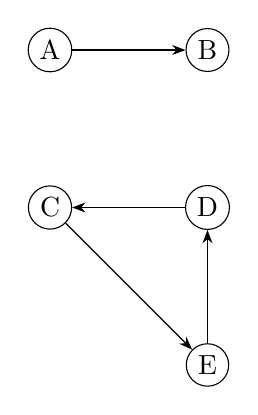
\begin{tikzpicture}[->,>=Stealth,node distance=2cm,on grid,auto]
	\node[circle, draw, inner sep=2pt] (A) {A};
	\node[circle, draw, inner sep=2pt] (B) [right=of A] {B};
	\node[circle, draw, inner sep=2pt] (C) [below=of A] {C};
	\node[circle, draw, inner sep=2pt] (D) [right=of C] {D};
	\node[circle, draw, inner sep=2pt] (E) [below=of D] {E};

	\draw (A) to (B);
	\draw (D) to (C);
	\draw (C) to (E);
	\draw (E) to (D);


\end{tikzpicture}



\end{document}
